\documentclass{beamer}
\usetheme{metropolis}

\usepackage[spanish]{babel}
\usepackage[utf8]{inputenc}
\usepackage{tikz}
\usepackage{xcolor}
\usepackage{amsmath}
\usepackage{listings}

% Definición de colores personalizados
\definecolor{primary}{RGB}{46, 204, 113}
\definecolor{secondary}{RGB}{52, 152, 219}
\definecolor{accent}{RGB}{231, 76, 60}
\definecolor{background}{RGB}{236, 240, 241}
\definecolor{gradient1}{RGB}{255, 107, 107}
\definecolor{gradient2}{RGB}{255, 159, 67}

% Configuración del tema
\setbeamercolor{normal text}{fg=black,bg=background}
\setbeamercolor{structure}{fg=primary}
\setbeamercolor{alerted text}{fg=accent}

\definecolor{lightgray}{rgb}{0.95,0.95,0.95}
\definecolor{darkgreen}{rgb}{0,0.5,0}
\definecolor{darkblue}{rgb}{0,0,0.5}

\lstset{
  backgroundcolor=\color{lightgray},
  basicstyle=\tiny\ttfamily,
  keywordstyle=\color{darkblue}\bfseries,
  commentstyle=\color{darkgreen},
  stringstyle=\color{red},
  numbers=left,
  numberstyle=\tiny\color{gray},
  stepnumber=1,
  numbersep=5pt,
  showspaces=false,
  showstringspaces=false,
  showtabs=false,
  frame=single,
  tabsize=2,
  language=Python,
  breaklines=true,
  breakatwhitespace=true
}

\graphicspath{{./images/}}

\title{\Huge\textbf{Inventarios}}
\author{Investigación Operativa}
\date{}

\begin{document}

\begin{frame}
    \titlepage
    \begin{tikzpicture}[remember picture,overlay]
        \node[anchor=south west,inner sep=30pt] at (current page.south west) {
            
\includegraphics[height=1cm]{../misc/UdeSA.png}
        };
    \end{tikzpicture}
\end{frame}

\begin{frame}{Objetivos de la Clase Práctica}
    \begin{itemize}
        \item<1-> Aplicar el modelo EOQ en situaciones reales
        \item<2-> Calcular costos totales de inventario
        \item<3-> Determinar puntos de reorden óptimos
        \item<4-> Analizar casos con descuentos por cantidad
    \end{itemize}
\end{frame}

\begin{frame}{Variables del Modelo EOQ}
    \begin{columns}[T]
        \begin{column}{0.5\textwidth}
            \begin{itemize}
                \item \textcolor{primary}{D} = Demanda
                \item \textcolor{primary}{Q} = Cantidad a pedir
                \item \textcolor{primary}{h} = Costo de mantener
            \end{itemize}
        \end{column}
        \begin{column}{0.5\textwidth}
            \begin{itemize}
                \item \textcolor{primary}{K} = Costo de pedir
                \item \textcolor{primary}{CT} = Costo total
                \item \textcolor{primary}{L} = Lead time
            \end{itemize}
        \end{column}
    \end{columns}
\end{frame}

\begin{frame}{Fórmulas Clave}
    \begin{alertblock}{Cantidad Económica de Pedido (EOQ)}
        \vspace{0.2cm}
        \[ Q^* = \sqrt{\frac{2KD}{h}} \]
    \end{alertblock}
    \pause
    \begin{block}{Costo Total}
        \vspace{0.2cm}
        \[ CT = \frac{hQ}{2} + \frac{KD}{Q} \]
    \end{block}
    \pause
    \begin{block}{Número de Pedidos y Tiempo entre Pedidos}
        \vspace{0.2cm}
        \[ N^* = \frac{D}{Q^*} \qquad T^* = \frac{Q^*}{D} \]
    \end{block}
\end{frame}

\begin{frame}{Ejercicio 1: EOQ Básico}
    \begin{block}{Datos}
        \begin{itemize}
            \item Demanda anual: 1200 unidades
            \item Costo de ordenar: \$500 por orden
            \item Costo de mantener: \$100 por unidad/año
        \end{itemize}
    \end{block}
    \pause
    \begin{alertblock}{¿Qué debemos calcular?}
        \begin{enumerate}
            \item Cantidad óptima de pedido (Q*)
            \item Costo total anual (CT)
            \item Número de pedidos por año (N*)
            \item Tiempo entre pedidos (T*)
        \end{enumerate}
    \end{alertblock}
\end{frame}

\begin{frame}{Resolución Ejercicio 1}
    \begin{columns}[T]
        \begin{column}{0.5\textwidth}
            \textcolor{primary}{Cantidad óptima:}
            \[ Q^* = \sqrt{\frac{2(500)(1200)}{100}} = 110 \]
            \vspace{0.5cm}
            \textcolor{primary}{Costo total:}
            \[ CT = \frac{100(110)}{2} + \frac{500(1200)}{110} \]
            \[ CT = \$10,954.55 \]
        \end{column}
        \begin{column}{0.5\textwidth}
            \textcolor{primary}{Número de pedidos:}
            \[ N^* = \frac{1200}{110} \approx 11 \]
            \vspace{0.5cm}
            \textcolor{primary}{Tiempo entre pedidos:}
            \[ T^* = \frac{110}{1200} \times 12 \approx 1.1 \text{ meses} \]
        \end{column}
    \end{columns}
\end{frame}

\begin{frame}{Gráfico del Ejercicio 1}
    \begin{figure}
        \centering
        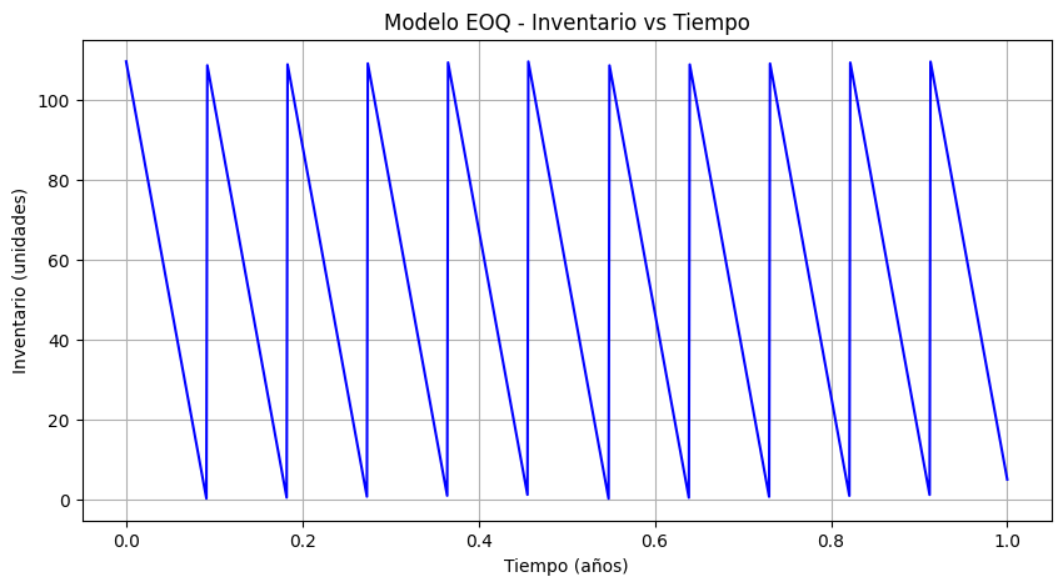
\includegraphics[width=\linewidth]{eoq_basico.png}
        \caption{Gráfico del inventario en función del tiempo}
    \end{figure}
\end{frame}

\begin{frame}{Ejercicio 2: Punto de Reorden}
    \begin{block}{Datos Adicionales}
        \begin{itemize}
            \item Lead time: 5 días
            \item Días laborables: 250 días/año
        \end{itemize}
    \end{block}
    \pause
    \begin{alertblock}{Punto de Reorden (R)}
        \vspace{0.2cm}
        \[ R = \text{Demanda diaria} \times \text{Lead time} \]
        \[ \text{Demanda diaria} = \frac{12000}{250} = 48 \text{ unidades/día} \]
        \[ R = 48 \times 5 = 240 \text{ unidades} \]
    \end{alertblock}
\end{frame}

\begin{frame}{Gráfico del Ejercicio 2}
    \begin{figure}
        \centering
        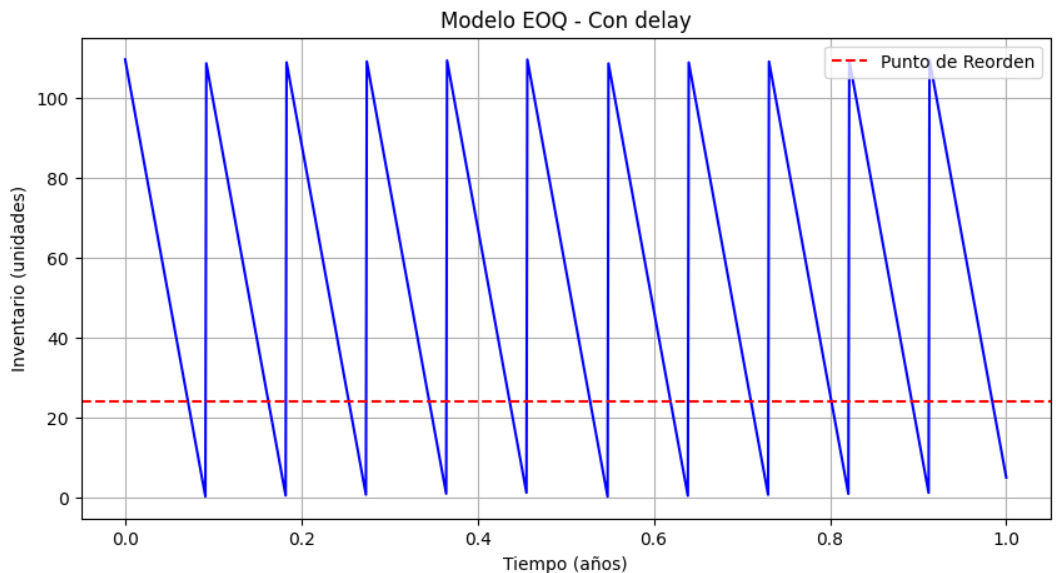
\includegraphics[width=\linewidth]{eoq_con_delay.png}
        \caption{Gráfico del inventario en función del tiempo}
    \end{figure}
\end{frame}

\begin{frame}{EOQ con perdidas}
    \begin{figure}
        \centering
        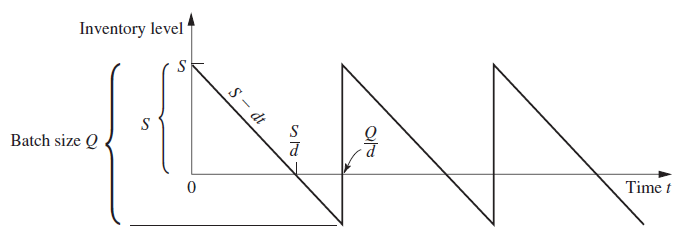
\includegraphics[width=\linewidth]{esquema_perdidas.png}
        \caption{Gráfico del inventario en función del tiempo}
    \end{figure}

\begin{itemize}
    \item Cuando ocurre un faltante, los clientes esperarán el tiempo necesario para satisfacer su demanda. Las ordenes demoradas se satisfacen instantáneamente cuando llegan los productos.
\end{itemize} 
\end{frame}

\begin{frame}{EOQ con perdidas}
\begin{itemize}
    \item \textcolor{primary}{p}: costo por unidad por unidad de tiempo perdido
\end{itemize}
    \begin{columns}[T]
        \begin{column}{0.5\textwidth}
            \textcolor{primary}{Cantidad óptima de compra:}
            \[ Q^* = \sqrt{\frac{2DK}{h}}\sqrt{\frac{p+h}{p}} \]
            \vspace{0.5cm}
            \textcolor{primary}{Tiempo de compra:}
            \[T^* = \frac{Q^*}{D}=\sqrt{\frac{2K}{Dh}}\sqrt{\frac{p + h}{p}}\]
        \end{column}
        \begin{column}{0.5\textwidth}
            \textcolor{primary}{Inventario luego de la compra:}
            \[ S^* = \sqrt{\frac{2DK}{h}}\sqrt{\frac{p}{p+h}} \]
            \vspace{0.5cm}
            \textcolor{primary}{Tiempo inventario positivo:}
            \[T_S^* = \frac{S^*}{D} = \sqrt{\frac{2K}{Dh}}\sqrt{\frac{p+h}{p}}\]
        \end{column}
    \end{columns}
\end{frame}

\begin{frame}{Ejercicio de la teorica}
Hagamos de cuenta que estamos en una empresa de televisores. El costo de abrir una línea de producción es de \$12000. Excluyendo este costo, cada unidad de sonido cuesta \$10 para producirse y \$0.3 para almacenarse. La línea de producción puede producir como mucho 8000 televisores por mes. El costo o multa por unidad que no se tiene es de 1,10. ¿Cuál es la cantidad óptima de unidades de sonido que deben hacerse y cada cuánto?
    \begin{itemize}
            \item p = 1,10
            \item K = 12000
            \item h = 0,30
            \item D = 8000
        \end{itemize}
\end{frame}

\begin{frame}{Ejercicio de la teorica}
    
    \begin{columns}[T]
        \begin{column}{0.5\textwidth}
            \textcolor{primary}{Cantidad óptima de compra:}
            \[ Q^* = \sqrt{\frac{2(8000)(12000)}{0.3} \cdot \frac{1.1+0.3}{1.1}}  \]
            \[= 28,540\,\text{unidades}\]
            \vspace{0.5cm}
            \textcolor{primary}{Tiempo de compra:}
            \[T^* = \frac{28540}{8000}= 3.6 \,\text{meses}\]
        \end{column}
        \begin{column}{0.5\textwidth}
            \textcolor{primary}{Inventario luego de la compra:}
            \[ S^* = \sqrt{\frac{2(8000)(12000)}{0.3} \cdot \frac{1.1}{1.1+0.3}}  \]
            \[= 22,424\,\text{unidades}\]
            \vspace{0.5cm}
            \textcolor{primary}{Tiempo inventario positivo:}
            \[T_S^* = \frac{22424}{8000} = 2.8 \,\text{meses}\]
        \end{column}
    \end{columns}
\end{frame}

\begin{frame}{Gráfico perdidas}
    \begin{figure}
        \centering
        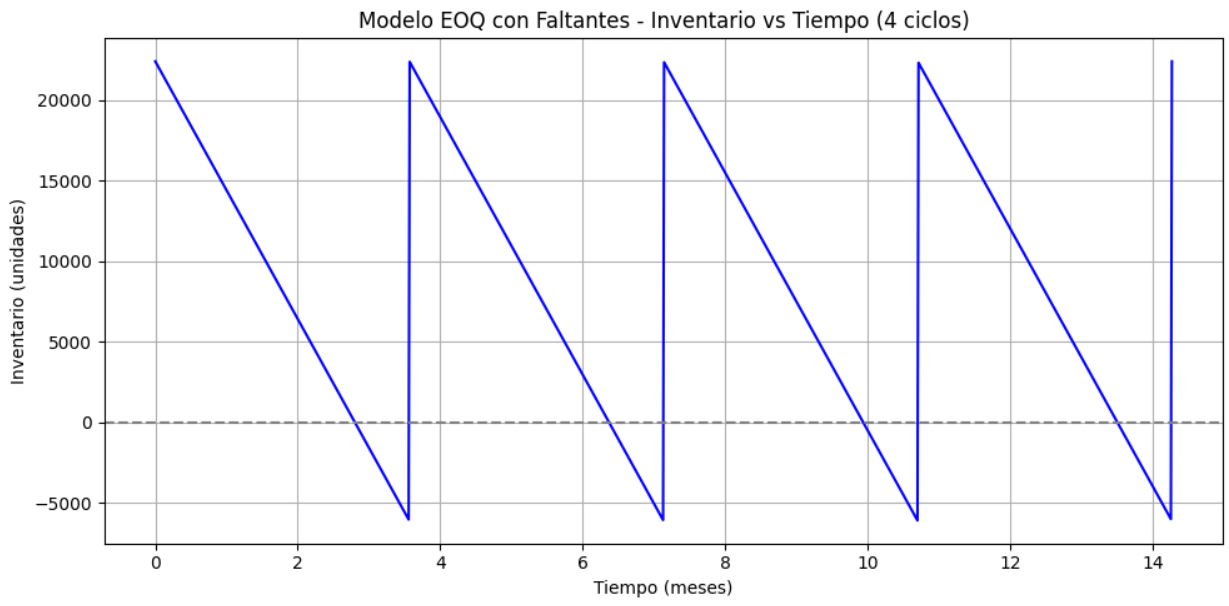
\includegraphics[width=\linewidth]{eoq_inventario_faltante.png}
        \caption{Gráfico del inventario en función del tiempo}
    \end{figure}
\end{frame}

\begin{frame}{Ejercicio 3: Descuentos por Cantidad}
    \begin{columns}[T]
        \begin{column}{0.6\textwidth}
            \begin{block}{Estructura de Descuentos}
                \begin{itemize}
                    \item 0-999: \$100/unidad
                    \item 1000-4999: \$95/unidad
                    \item 5000+: \$90/unidad
                \end{itemize}
            \end{block}
        \end{column}
        \begin{column}{0.4\textwidth}
            \begin{block}{Datos}
                \begin{itemize}
                    \item D = 5000
                    \item K = \$200
                    \item h = 20\% × \$ unidad
                \end{itemize}
            \end{block}
        \end{column}
    \end{columns}
\end{frame}


\begin{frame}{Metodología de Resolución}
    \begin{enumerate}
        \item Calcular Q* para cada precio
        \item Si Q* está en el rango válido, calcular CT
        \item Si Q* no está en el rango, evaluar los extremos
        \item Comparar todos los costos totales válidos
    \end{enumerate}
    \pause
    \begin{alertblock}{Recordar}
        El costo de mantener (h) cambia con cada precio:
        \[ h = 0.20 \times p \]
    \end{alertblock}
\end{frame}

\begin{frame}{Ejercicio 3: Resultados por Tramo de Descuentos}
    \begin{block}{Cálculos por Rango de Descuento}
        \begin{itemize}
            \item \textbf{0--999 unidades:} Precio = \$100, \quad $Q = 316.23$, \quad Costo Total = \$506{,}324.56
            \item \textbf{1000--4999 unidades:} Precio = \$95, \quad $Q = 1000.00$, \quad Costo Total = \$485{,}500.00
            \item \textbf{5000+ unidades:} Precio = \$90, \quad $Q = 5000.00$, \quad Costo Total = \$495{,}200.00
        \end{itemize}
    \end{block}
\end{frame}

\begin{frame}{Política Óptima}
    \begin{block}{Mejor decisión según Costo Total}
        \begin{itemize}
            \item Rango óptimo: \textbf{1000--4999 unidades}
            \item Precio unitario: \textbf{\$95}
            \item Cantidad óptima a pedir: \textbf{1000.00 unidades}
            \item Costo total anual: \textbf{\$485{,}500.00}
        \end{itemize}
    \end{block}
\end{frame}

\begin{frame}{Ejercicio Computadoras Thinkpad}
    Lenovo vende computadoras Thinkpad y, debido a su popularidad, se espera que este año la demanda llegue a 12000 unidades distribuida de manera constante durante el año. Cada vez que el local realiza un pedido al proveedor incurre en un costo fijo de \$500 por orden. El costo de mantener una computadora en inventario es de \$10 por unidad por mes.
\end{frame}

\begin{frame}{Item A - Consigna}
    ¿Cuál es la cantidad óptima a pedir y cada cuánto tiempo debería hacerse un nuevo pedido si no se permiten faltantes?
\end{frame}

\begin{frame}{Item A - Resolución}
\begin{align*}
Q &= \sqrt{\frac{2DK}{h}} = \sqrt{\frac{2 \cdot 12{,}000 \cdot 500}{120}} = 316.23 \\[2em]
T &= \frac{Q}{D} = \frac{316.23}{12{,}000} = 0.02635 \text{ años} \approx 9.62 \text{ días}
\end{align*}
\end{frame}

\begin{frame}{Item A - Gráfico}
\begin{figure}
    \centering
    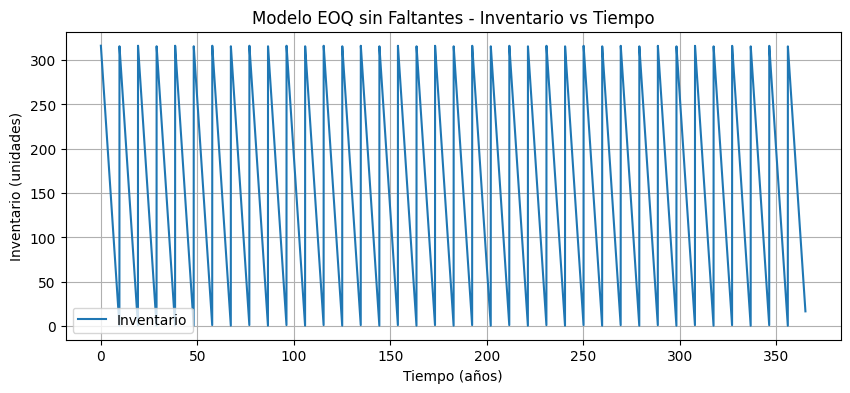
\includegraphics[width=\linewidth]{thinkpad_normal.png}
    \caption{Inventario en función del tiempo}
\end{figure}
\end{frame}

\begin{frame}{Item B - Consigna}
    Desde que se realiza el pedido hasta que llega, pasan 5 días. No se permite que falten computadoras en el inventario. ¿Cuál es el punto de reorden y cómo se comporta el inventario si se realiza el pedido en ese momento?
\end{frame}

\begin{frame}{Item B - Resolución}
    \begin{center}
        \textcolor{primary}{Punto de reorden:}
        \[ R = D \cdot L \]
        \[ R = 12{,}000 \cdot \frac{5}{365} \]
        \[ R = 164.38 \text{ unidades} \]
    \end{center}
\end{frame}

\begin{frame}{Ítem B - Gráfico}
    \begin{figure}
        \centering
        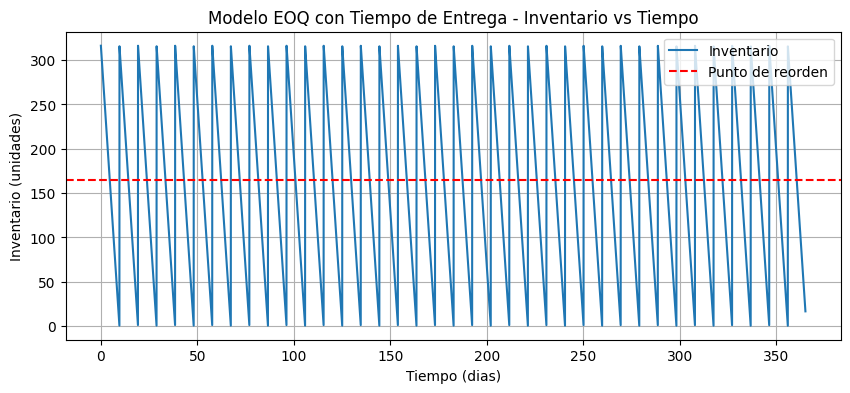
\includegraphics[width=\linewidth]{thinkpad_lead.png}
        \caption{Comportamiento del inventario con lead time}
    \end{figure}
\end{frame}

\begin{frame}{Item C - Consigna}
    Si se sabe que, ante un faltante de inventario, la pérdida económica por cliente no atendido se estima en \$900 por unidad, se permite que exista escasez en ciertos momentos del ciclo. ¿Cómo cambian la cantidad óptima a pedir, el nivel máximo de inventario y la cantidad máxima de faltantes permitidos?
\end{frame}

\begin{frame}{Ítem C - Resolución}
\begin{align*}
Q &= \sqrt{\frac{2DK}{h} \cdot \frac{h + p}{p}} \\
  &= \sqrt{100{,}000 \cdot \frac{1{,}020}{900}} \\
  &= 336.54 \text{ unidades} \\[1em]
S &= Q \cdot \frac{p}{p + h} \\
  &= 336.54 \cdot \frac{900}{1{,}020} \\
  &= 296.03 \text{ unidades} \\[1em]
\end{align*}
\end{frame}

\begin{frame}{Ítem C - Resolución}
\begin{align*}
T &= \frac{Q}{D} \\
  &= \frac{336.54}{12{,}000} \\
  &= 0.0280 \text{ años} \approx 10.22 \text{ días} \\[1em]
\text{Faltantes máx.} &= Q - S \\
  &= 336.54 - 296.03 \\
  &= 40.51 \text{ unidades}
\end{align*}
\end{frame}

\begin{frame}{Ítem C - Gráfico}
\begin{figure}
    \centering
    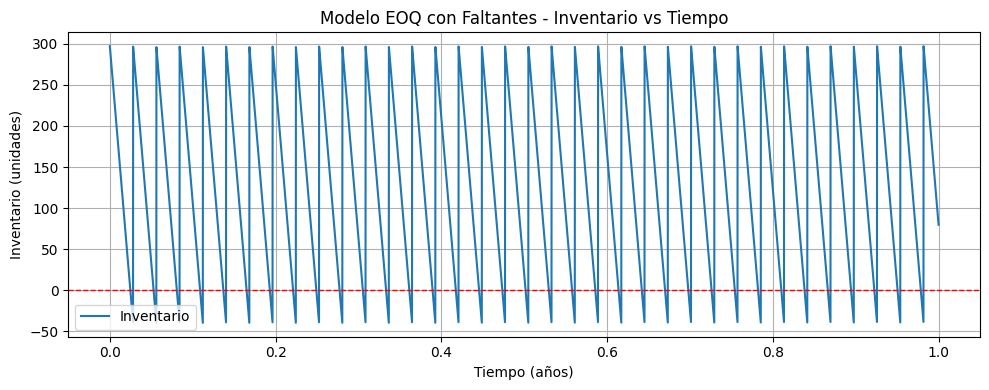
\includegraphics[width=\linewidth]{thinkpad_perdidas.png}
    \caption{Inventario en función del tiempo}
\end{figure}
\end{frame}

\begin{frame}{Ítem D - Consigna}
    Se sabe que a partir del mes de octubre la demanda aumenta en un 25\% y pero debido a su consumo se logra reducir el costo de produccion en un 50\% ¿Cómo cambian las cantidad de pedidos necesarios y los tiempos en los que se hacen los mismos?
\end{frame}


\begin{frame}{Ítem D - Resolución}
    \textbf{Antes del mes 10:}
    \begin{align*}
    Q_1 &= \sqrt{\frac{2 \cdot 12{,}000 \cdot 500}{120}} = 316.23 \\
    T_1 &= \frac{316.23}{12{,}000} = 0.02635 \text{ años} \approx 9.62 \text{ días}
    \end{align*}

    \vspace{1em}
    \textbf{A partir del mes 10 (día 300):}
    \begin{itemize}
        \item Nueva demanda: $D_2 = 15{,}000$
        \item Nuevo costo por orden: $K_2 = 250$
    \end{itemize}
    \begin{align*}
    Q_2 &= \sqrt{\frac{2 \cdot 15{,}000 \cdot 250}{120}} = 250.00 \\
    T_2 &= \frac{250}{15{,}000} = 0.01667 \text{ años} \approx 6.08 \text{ días}
    \end{align*}
\end{frame}

\begin{frame}{Ítem D - Gráfico}
\begin{figure}
    \centering
    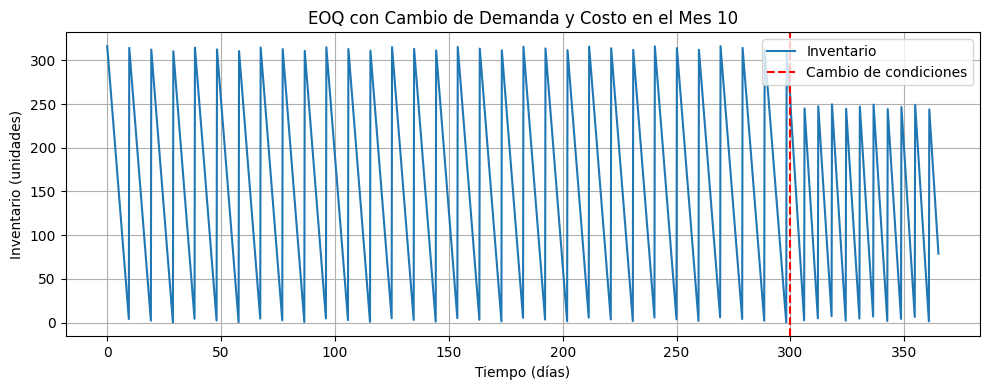
\includegraphics[width=\linewidth]{thinkpad_cambio_demanda.png}
    \caption{Inventario en función del tiempo}
\end{figure}
\end{frame}

\begin{frame}{Terminamos}
    \begin{center}
        \Large{\textbf{¿Dudas?\\¿Consultas?}}
    \end{center}
    \begin{tikzpicture}[remember picture,overlay]
        \node[anchor=south,inner sep=30pt] at (current page.south) {
            
\includegraphics[height=1cm]{../misc/UdeSA.png}
        };
    \end{tikzpicture}
\end{frame}

\end{document}
